\documentclass[sigconf]{acmart}
\setcopyright{none}
\settopmatter{printacmref=false,printccs=false,printfolios=true}
\renewcommand\footnotetextcopyrightpermission[1]{}
\acmConference[SymDiv Fall 2026]{SymDiv Advanced Topics in Program Analysis}{Fall 2026}{Singapore}
\acmYear{2026}
\copyrightyear{2026}
\usepackage{booktabs}
\usepackage{listings}
\usepackage{tikz}
\usetikzlibrary{arrows.meta,positioning}
\usepackage{xcolor}
\emergencystretch=3em
\raggedbottom
\lstset{language=C,basicstyle=\ttfamily\footnotesize,columns=fullflexible,keepspaces=true,breaklines=true,frame=single,showstringspaces=false,aboveskip=6pt,belowskip=6pt}
% Generated from results; do not edit.
\newcommand{\AbstractResults}{The hybrid, model-only, and symbolic-only systems classify all 24 files correctly in each stratum. CSA recalls 9 of 12 pilot positives and 6 of 12 Juliet positives, with no false positives. Thus the evaluation does not demonstrate an accuracy advantage from adding the LLM to this symbolic subset.}
\newcommand{\ResultsDiscussion}{Table~\ref{tab:classification} gives all confusion matrices. On the pilot, CSA obtains 9 TP, 0 FP, 12 TN, and 3 FN (75\% recall and 85.7\% F1). On Juliet it obtains 6 TP, 0 FP, 12 TN, and 6 FN (50\% recall and 66.7\% F1). SymDiv v2 obtains 12 TP, 0 FP, 12 TN, and 0 FN in each stratum. Its precision, recall, F1, and accuracy are therefore 100\% for these files. No analyzer or provider execution failed in either final run.}
\newcommand{\AblationDiscussion}{Both LLM-only and symbolic-only have exactly the same file predictions as SymDiv v2 on both strata. The source gate changes zero natural model classifications: all proposed bug sites have valid witnesses, while negative sites are model-safe. Consequently these primary runs show neither an accuracy gain from verification nor an accuracy gain from adding the model to the supported symbolic subset.}
\newcommand{\DispositionDiscussion}{Table~\ref{tab:dispositions} reports 12 accepted and 12 model-safe pilot sites. Juliet has 12 accepted and 32 model-safe sites, reflecting its multi-helper good branches. The hybrid has no refuted, inconclusive, unknown, missing, or invalid proposals in these two runs. Symbolic-only refutes 10 pilot sites and records two inconclusive outcomes: one timeout on the unsigned bitwise case and one loop-bound exhaustion on the guarded loop. It refutes all 32 negative Juliet sites. Its 100\% warning accuracy on the pilot therefore must not be called 100\% proof coverage.}
\newcommand{\CostDiscussion}{The final Juliet run used 425,535 input and 4,648 output tokens, totaling 430,183, below its 500,000-token ceiling. The 24 requests took 236.214 seconds in aggregate, with median 9.790 seconds and inclusive-quartile IQR 3.237 seconds. Its entire comparison harness took 241.062 seconds. The separate smoke test used 17,913 tokens and is excluded from these primary-run totals. The pilot preserves its original 406,811-token model record, while v2 replay used zero new model calls. The recorded environment is macOS 26.1 on arm64, Python 3.9.6, Z3 4.13.3, and Apple Clang 17.0.0. Pilot responses record Codex CLI 0.153.4; new Juliet responses record 0.155.0-alpha.16.4.}
\newcommand{\ExternalCases}{All six external CSA false negatives are the random-input bad branches: \texttt{j002}, \texttt{j006}, \texttt{j016}, \texttt{j018}, \texttt{j019}, \texttt{j022}. They cover all six retained flow variants. CSA detects each fixed-zero bad branch and emits no warning for any good branch. SymDiv, LLM-only, and symbolic-only recover the random-input cases under the declared nondeterministic input model. All systems therefore have true-positive and true-negative examples; CSA also has the listed false negatives. There are no observed false positives in either stratum and no hybrid false negatives, so examples in those absent categories cannot honestly be supplied. Zero categories are reported explicitly rather than filled with fabricated incidents.}
\newcommand{\RegressionSummary}{The final regression suite passes 62 tests. In addition, all 24 accepted hybrid witnesses (12 per stratum) were replayed in compiled C with Clang\,\texttt{-fsanitize=undefined} at optimization level zero. Every execution produced an integer division-by-zero diagnostic at the recorded target line. The harness supplies recorded parameters and random-call values; this validates concrete paths under the declared library-input model, not the existence of a real libc random seed.}
\newcommand{\ReproductionSummary}{A clean Git clone with a newly created virtual environment passed all 62 tests, regenerated the 24 Juliet files byte for byte, reproduced every file prediction and site disposition in both strata without a new model call, and rebuilt the PDF. This was an isolated checkout on the same machine and compiler, not a reproduction by a second person or on a different platform.}
\newcommand{\ConclusionResults}{On the retained subjects, the hybrid achieves perfect warning classification, but so do its LLM-only and symbolic-only ablations. The supported symbolic subset already explains the recovered CSA misses. The evidence supports the corrected acceptance boundary and reproducible case analysis; it does not demonstrate a necessary neural contribution or a production-scale advantage.}

\title{SymDiv: Source-Grounded Verification of Neural Divide-by-Zero Hypotheses in C}
\author{SymDiv Project}


\begin{document}
\begin{abstract}
A satisfiable language-model hypothesis need not describe an execution of the
program it purports to analyze. This project studies that distinction for
integer division- and remainder-by-zero detection in C. The initial SymDiv
prototype checked only model-proposed predicates and a zero denominator; a
correctness audit showed that omitted guards and assignments could turn safe
programs into apparently verified findings. SymDiv v2 instead constructs
independent, bounded source paths, models a restricted set of 32-bit C integer
operations, and accepts a neural proposal only when the complete source formula
admits a zero-denominator witness. We compare Clang Static Analyzer (CSA),
model-only predictions, the repaired hybrid, and its symbolic-only component
on 24 handcrafted programs and 24 independently sourced, label-blinded Juliet
programs. The latter contain 44 division sites. Pilot neural responses are
replayed; Juliet responses are newly collected under a frozen budget.
\AbstractResults{}
We report all dispositions and costs, preserve the original pilot, and include
regressions that test the original unsound acceptance rule. The contribution is
an inspectable and reproducible exploratory comparison, including the limits
of what its favorable classification scores establish.
\end{abstract}
\maketitle

\section{Introduction}
Static analysis must connect a reported defect to the semantics of the program.
A language model may recognize that a denominator can be zero, but it can also
omit an early return, forget an assignment, or confuse an entry-state variable
with its value after a loop. Adding an SMT solver does not automatically repair
these mistakes. The solver proves a property of the supplied formula, not that
the formula is a faithful translation of the source.

This project makes the problem concrete using integer division and remainder
in C. The task is narrow enough to inspect each warning, but includes control
flow, arithmetic relationships, mutable local variables, loops, and library
input. The traditional comparison tool is the executable Clang Static Analyzer
with its \texttt{core.DivideZero} checker. The proposed analyzer, SymDiv, asks a
language model for a candidate verdict and explicit predicates, then uses a
separately implemented symbolic stage to decide whether to emit a warning.

The first implementation, called v1 here, had a consequential defect. It
required the proposed denominator text to match the source, but did not
independently encode how execution reached that denominator. For a local
variable initialized to seven, an unconstrained symbolic variable with the
same name could still be assigned zero. A 100\% score on 24 simple handcrafted
examples failed to reveal this defect because the model happened to produce
correct classifications. Thus aggregate accuracy and a formally satisfiable
formula were insufficient evidence for the advertised verification boundary.

Version 2 repairs this boundary. It derives environments and path constraints
from the Clang AST, accounts for assignments and early exits, and checks a
neural proposal against reachable states at its actual division site. It also
repairs incomplete-run scoring and location-dependent replay identifiers. These
changes are recorded as a separate experiment, rather than silently replacing
the original pilot. A new evaluation uses a deterministic subset of the NIST
Juliet suite, with the original archive checksum and derived sources retained.

Three questions guide the study. RQ1 asks how the four systems classify the
same programs under the declared task. RQ2 asks what the neural and symbolic
parts contribute separately, including whether source grounding actually changes
observed model decisions. RQ3 asks what limitations, failure modes, and resource
costs remain. The study does not attempt a new state-of-the-art whole-program C
analyzer or a large-scale benchmark ranking. Its scope is a small experimental
artifact whose claims can be checked against source, responses, and witnesses.

The contributions are a reproducible v1 counterexample, a source-grounded
acceptance mechanism, and a comparison separating independent subjects,
ablations, and diagnostic regressions. Negative findings about the neural
component are retained.

\section{Task and Comparison Boundary}
\subsection{Analysis question}
A program is positive when some admitted function input or modeled library
input reaches an eligible integer division or remainder with denominator zero,
without prior undefined arithmetic on that path. The four recognized syntactic
operators are \texttt{/}, \texttt{\%}, \texttt{/=}, and \texttt{\%=}. Floating-point
division is excluded. Each pilot file has one site; a Juliet good-branch file
may have several. In both strata a file-level warning means that at least one
eligible site receives a warning. Site counts describe workload and dispositions,
while the confusion matrices use files as the unit of observation.

The experimental machine uses 32-bit \texttt{int} and \texttt{unsigned int}.
Signed arithmetic paths whose computed values are outside the representable
range are excluded. Unsigned arithmetic wraps modulo $2^{32}$. The supported
conversion from unsigned to signed follows the tested Clang target's
two's-complement behavior. Integer quotient and remainder are implemented with
truncation toward zero and the associated remainder identity, rather than
using SMT integer division directly as a C operation~\cite{c11,z3-arithmetic}.
The analysis is deliberately target-specific; this is not a portable model of
every implementation-defined C behavior.

Functions containing sites are analyzed as entries with arbitrary admitted
scalar parameters. No general calling-context, heap, or alias analysis is
claimed. In the selected Juliet subjects, the site-bearing functions have no
parameters, and the retained public good wrapper calls its helper functions.
The arbitrary-entry convention therefore does not discard a caller-provided
precondition in this subset. General projects would require call summaries or
additional exclusions before inheriting this evaluation protocol.

\subsection{Baseline policy and fairness}
CSA is run once per file using C11, SARIF output, and
\texttt{-analyzer-checker=core.DivideZero}. This enables the target checker;
it does not disable every other default checker. Only division-by-zero
diagnostics are counted. The command, return code, stderr, normalized findings,
and tool version are retained. A missing SARIF report, nonzero return code, or
timeout is an execution failure, never a negative classification.

The comparison has an important policy boundary. Clang documents that the core
checker warns when it can prove a denominator is zero. Its separate tainted-division
checker is more pessimistic about potentially attacker-controlled
values~\cite{clang-checkers}. Our existential label can therefore count a
possible-zero parameter as positive even when \texttt{core.DivideZero} declines
to warn. Such a result is reported as a false negative under this benchmark's
labels, but it is not evidence that all symbolic analysis is incapable of the
reasoning. We keep this declared baseline fixed rather than tune its options
after observing misses.

\section{Source-Grounded Approach}
\subsection{Representation and extraction}
Clang is used as a parser, separately from its static analyzer. JSON AST
extraction records the enclosing function, operator, exact denominator text,
line, byte column, and function source. Both ordinary binary operators and
compound assignments are considered, with integer-type filtering. UTF-8 source
slices use byte offsets, matching Clang's locations. A site identifier hashes
source content, function, position, and operator. It deliberately excludes the
absolute checkout path, so an unchanged subject keeps its identifier after
relocation. Unmaterialized preprocessing directives and AST macro expansions
are rejected; the Juliet importer supplies preprocessed source before analysis.

The source hash also guards replay. A stored response is accepted for replay
only when the subject bytes match. For historical v1 responses, old site IDs are
mapped to current IDs by the recorded function, location, operator, denominator,
and exact function text. The migration first checks the pilot source against
the archived v1 commit. This is transport migration of recorded predictions,
not a fresh model evaluation. Altered source must not inherit a cached verdict
merely because the filename is unchanged.

\begin{figure}[t]
\centering
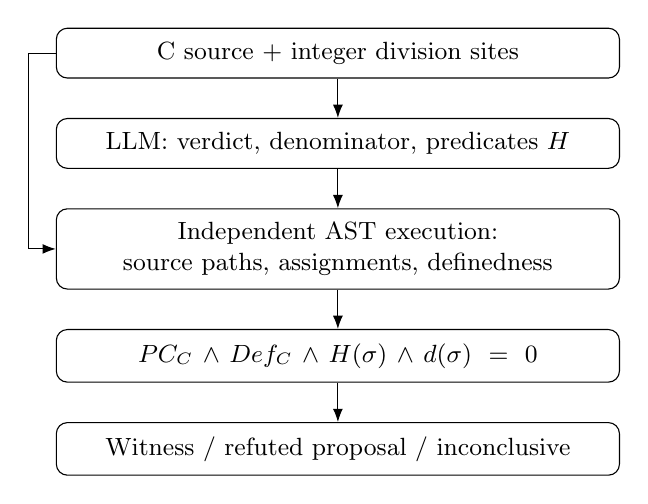
\begin{tikzpicture}[node distance=5mm,box/.style={draw,rounded corners,align=center,font=\small,text width=6.8cm,inner sep=5pt},>=Latex]
\node[box] (c) {C source + integer division sites};
\node[box,below=of c] (llm) {LLM: verdict, denominator, predicates $H$};
\node[box,below=of llm] (exec) {Independent AST execution:\\source paths, assignments, definedness};
\node[box,below=of exec] (query) {$PC_C \land Def_C \land H(\sigma) \land d(\sigma)=0$};
\node[box,below=of query] (out) {Witness / refuted proposal / inconclusive};
\draw[->] (c.west) -- ++(-0.35,0) |- (exec.west);
\draw[->] (c)--(llm); \draw[->] (llm)--(exec); \draw[->] (exec)--(query); \draw[->] (query)--(out);
\end{tikzpicture}
\caption{The v2 acceptance boundary. Source execution supplies constraints
independently of the model. Neither a model confidence score nor satisfiability
of an ungrounded hypothesis is sufficient.}
\label{fig:architecture}
\end{figure}

\subsection{Neural interface}
Each request contains one complete, label-blinded C file and its extracted
sites. The unchanged pilot prompt requests \texttt{bug}, \texttt{safe}, or
\texttt{unknown} for every site; simple predicates; the exact denominator text;
a short rationale; and a confidence score. Confidence is logged but never
used as a warning threshold. Duplicate or unexpected site IDs invalidate the
response, while an omitted site is retained as a missing hypothesis.

The primary provider is the locally authenticated Codex CLI, requesting
\texttt{gpt-5.6-sol} at medium reasoning effort. The harness uses an ephemeral
read-only session with a JSON output schema. It invokes the model from an empty
temporary working directory, removes API-key variables from the child
environment, and instructs it to use only the supplied source. A returned tool
execution invalidates the experiment protocol. The artifact retains structured
responses, event streams, reported usage, latency, requested model, and CLI
version. The requested model name is not a guarantee that the hosted service's
weights will remain unchanged over time.

A \texttt{safe} verdict suppresses a candidate; it is not a proof of safety.
Likewise, \texttt{unknown} is an abstention. This asymmetric interface means that
source verification can reject an incorrect positive but cannot recover a true
bug that the model never proposes. The symbolic-only ablation explicitly tests
what is lost by this candidate filter.

\subsection{Independent bounded execution}
An execution state contains a mapping from Clang declaration IDs to symbolic
values, the names currently in lexical scope, path constraints, initial inputs,
and a control-flow status. Declaration IDs prevent an inner variable from
accidentally replacing an outer variable of the same name. An assignment
updates the stored expression. Branches fork states with the condition or its
negation. Returns, breaks, and continues affect subsequent statement execution;
short-circuit and conditional expressions retain their activation conditions.

The interpreter supports scalar integer declarations and assignments,
comparisons, arithmetic, selected bitwise operations and casts, nested blocks,
conditionals, and bounded \texttt{while}, \texttt{for}, and \texttt{do} loops.
Unsigned shifts are constrained to valid shift amounts. It rejects pointer
operations, arbitrary local calls, mutable globals, mutable static locals,
uninitialized reads, unsupported types, and embedded mutation with unsupported
evaluation order. Compound assignments requiring a different promoted result
type also abstain, and printing summaries require the declared void interface.
A local function called \texttt{rand} is not automatically
treated as the library primitive. These restrictions are implementation
boundaries, not classifications of the programs as safe.

The Juliet compatibility interface models external \texttt{rand()} calls as
independent values in $[0,2^{31}-1]$ and printing as observation without relevant
state mutation. The upstream random-value macros themselves are preserved,
including their unsigned bitwise operations. This models nondeterministic
library input for defect reachability. It does not reconstruct a concrete libc
pseudo-random generator, infer a seed, or prove that an arbitrary sequence of
modeled values occurs for some real generator seed.

Exploration is limited to eight loop iterations and 4,096 statement-state
visits per function. A feasible continuation beyond a bound is retained as an
incompleteness reason. Pruning queries have a short timeout: UNSAT prunes a
path, while unknown keeps it with all its constraints. Consequently a pruning
timeout is not itself loss of coverage. Final acceptance queries have a
5,000\,ms timeout. Bound exhaustion, unsupported behavior, and final solver
unknown remain visible when no witness is found.

\subsection{Acceptance formula and witness meaning}
For a reached site $s$ on path $\pi$, let $\sigma_\pi$ be the environment at the
site, $PC_C$ its source-derived branch constraints, and $Def_C$ the constraints
excluding prior undefined arithmetic. Let $H$ denote the model's predicates.
The acceptance query is
\begin{equation}
 PC_C(\pi) \land Def_C(\pi) \land H(\sigma_\pi)
 \land d_s(\sigma_\pi)=0.
\end{equation}
The denominator is evaluated from the AST, not replaced by a fresh variable
with the same spelling. Model predicates bind to values in scope \emph{at the
site}; an invented identifier is rejected. This interpretation is especially
important for assignments and loops. A proposal written about entry values may
be rejected if it does not correctly describe the reached state.

At a division site, the zero-denominator query is recorded before adding the
nonzero condition needed to continue execution. Therefore a warning may refer
to that operation, but a later warning cannot rely on executing through an
earlier division by zero. Signed overflow and the unrepresentable signed
minimum divided by minus one are handled as prior undefined arithmetic for
subsequent execution.

Before the general solver, a fixed, small set of concrete input vectors is
substituted into the full formula: all zero, all one, all minus one, and up to
32 coordinate vectors with value one or minus one. A candidate is accepted
only if simplification makes the complete formula true. This is an inexpensive
witness search, not an inference that failure of these seeds establishes
safety. Otherwise Z3 is queried normally. Accepted results retain both initial
input values and values at the site.

A SAT result establishes a witness in this bounded, explicitly modeled subset.
It is not a machine-checked soundness theorem for the interpreter or arbitrary
C. UNSAT for all explored states refutes the \emph{proposal} only when
exploration is complete. If any relevant path remains unsupported or bounded,
the result is inconclusive. Even a refuted proposal need not prove safety when
its extra neural predicates exclude a different feasible bug path.

\section{Study Design and Artifact Controls}
\subsection{Subjects and independent provenance}
\begin{table}[t]
\caption{Evaluation strata. Labels and confusion matrices are file-level;
site counts measure extracted integer operations.}
\label{tab:subjects}
\centering\small
\begin{tabular}{lrrrr}\toprule
Stratum & Files & Positive & Negative & Sites\\\midrule
Handcrafted pilot & 24 & 12 & 12 & 24\\
Juliet derived subset & 24 & 12 & 12 & 44\\\bottomrule
\end{tabular}
\end{table}
The pilot contains constants, zero guards, contradictory branches, affine and
relational constraints, assignments, remainder, bitwise syntax, and loops.
It was designed for this project and is a development stratum, not an
independent generalization test. Its original model run and original results
remain under \texttt{results/pilot/}. The repaired method reuses those exact
neural responses and records new verification results separately.

The external stratum is derived from the official NIST Juliet C/C++ 1.3
archive~\cite{juliet}. The importer verifies the published SHA-256 before
extracting 12 C files from CWE-369. Selection uses the zero and random source
families and flow variants 01, 03, 06, 16, 17, and 31. Variants 01, 06, and 17
use division; variants 03, 16, and 31 use remainder. Each upstream file yields
one bad branch and one complete good branch. No subject is excluded after
observing predictions.

The branches are materialized by the preprocessor with a committed minimal
header. Comments are removed, label-bearing identifiers are renamed, diagnostic
strings are replaced with a neutral message, and a fixed shuffle assigns
neutral file IDs. The model receives neither filenames nor provenance labels.
The original random macros are checked against the archive's support header
and preserved exactly. Good helper functions remain in the program; this is
why the negative subset has more sites than files. Both analyzers receive the
same generated bytes. Raw upstream files, checksums, the provenance mapping,
preprocessing flags, and the generated manifest are included in the artifact.

Labels follow the upstream bad/good branch distinction under the declared
input model. Transformation review checks that arithmetic and guards are
preserved; compilation and extraction validate all files. This review was
AI-assisted. An independent human audit of every label is not claimed, and
Juliet provenance does not make the derived set a sample of real production
software. Structural similarity among variants also limits the effective
diversity of the 24 files.

\subsection{Configurations, budgets, and timing}
The v2 implementation, prompt, manifest, and external configuration were
committed before the primary external run at \texttt{0e4ea8f}. The archival v1
snapshot is \texttt{7ccbe06}; that snapshot was created during the repair work
and is not evidence of a pre-pilot commit. A dated protocol amendment records
why source grounding replaces the earlier acceptance rule. Subsequent delivery
checks added conservative rejection of out-of-contract inputs and retained
explicit replay-ID mappings. These changes did not alter any primary subject
or neural response; full replay with the delivered code checks every reported
classification and disposition.

A separate one-case smoke test used 17,913 reported tokens. Before the primary
run, its costly repeated feasibility queries motivated short pruning timeouts
and the generic concrete-seed optimization. The primary budget remained 24
calls and 500,000 tokens, with no retries and a 300-second per-call timeout.
Calls stop before exceeding the call limit or when the known token budget is
exhausted. A completed call may cross the token ceiling; such an overrun is
saved rather than discarded. Failed calls with unavailable usage stop further
calls because their remaining budget cannot be established reliably.

The primary environments and exact measured totals are generated from run files
in Table~\ref{tab:costs}. Python, Z3, Clang, OS, prompt hash, source hashes,
configuration, timestamps, and code hashes are recorded. Token totals are
CLI-reported usage, not C-source token counts or a monetary cost estimate.
Pilot model cost is historical; replay consumes no new model tokens. Neural
request latency and the local replay/verification harness time are reported
separately. The v2 harness also executes symbolic-only queries, so its end-to-end
wall time is an experimental-workflow cost rather than a clean standalone
hybrid-analyzer timing.

\subsection{Systems, metrics, and failure accounting}
Four systems use the same subjects. CSA counts matching static-analyzer
warnings. LLM-only counts any model \texttt{bug} verdict before verification.
SymDiv counts any source-grounded accepted neural proposal. Symbolic-only uses
the same execution engine with an empty hypothesis at every site, bypassing
neural candidate selection. The last two share implementation and are ablations,
not independent external tools. The symbolic-only pass runs in the comparison
harness; its predictions do not enter the model prompt.

For each system we compute TP, FP, TN, FN, precision, recall, F1, and accuracy.
Warning-based confusion matrices count an abstention as no warning, so an
inconclusive result on a positive is a false negative. The disposition table
makes these abstentions explicit; a true negative in the warning matrix must
not be described as a proof of safety. Execution failures are different: full
cohort scoring refuses missing, duplicate, unexpected, incomplete, or
non-Boolean predictions. An empty output cannot obtain credit for negative
subjects. Per-case checkpoints are written atomically after each completed or
failed attempt.

This descriptive study uses a small, correlated sample and one external
model call per subject. We report counts and explanations, not statistical
significance or confidence intervals for a real-world program population.

\section{Results and Ablations}
\begin{table*}[t]
\caption{File-level warning classification. Pilot neural predictions are replayed historical responses; Juliet uses fresh model calls. An inconclusive site emits no warning and is reported separately.}
\label{tab:classification}
\centering\small
\begin{tabular}{llrrrrrrrr}\toprule
Stratum & System & TP & FP & TN & FN & Precision & Recall & F1 & Accuracy\\\midrule
Pilot & Clang CSA & 9 & 0 & 12 & 3 & 100.0\% & 75.0\% & 85.7\% & 87.5\%\\
Pilot & LLM-only & 12 & 0 & 12 & 0 & 100.0\% & 100.0\% & 100.0\% & 100.0\%\\
Pilot & SymDiv v2 & 12 & 0 & 12 & 0 & 100.0\% & 100.0\% & 100.0\% & 100.0\%\\
Pilot & Symbolic-only & 12 & 0 & 12 & 0 & 100.0\% & 100.0\% & 100.0\% & 100.0\%\\
\midrule
Juliet & Clang CSA & 6 & 0 & 12 & 6 & 100.0\% & 50.0\% & 66.7\% & 75.0\%\\
Juliet & LLM-only & 12 & 0 & 12 & 0 & 100.0\% & 100.0\% & 100.0\% & 100.0\%\\
Juliet & SymDiv v2 & 12 & 0 & 12 & 0 & 100.0\% & 100.0\% & 100.0\% & 100.0\%\\
Juliet & Symbolic-only & 12 & 0 & 12 & 0 & 100.0\% & 100.0\% & 100.0\% & 100.0\%\\
\bottomrule\end{tabular}
\end{table*}
\begin{table}[t]
\caption{Site dispositions. H is the hybrid gate; S is symbolic-only. Model-safe is not a source safety proof.}
\label{tab:dispositions}
\centering\small
\begin{tabular}{lrrrr}\toprule
Outcome & Pilot H & Pilot S & Juliet H & Juliet S\\\midrule
Accepted witness & 12 & 12 & 12 & 12\\
Model-safe & 12 & 0 & 32 & 0\\
Refuted proposal & 0 & 10 & 0 & 32\\
Inconclusive & 0 & 2 & 0 & 0\\
Model-unknown & 0 & 0 & 0 & 0\\
Missing & 0 & 0 & 0 & 0\\
Invalid & 0 & 0 & 0 & 0\\
\bottomrule\end{tabular}
\end{table}
\begin{table}[t]
\caption{Measured costs. Pilot model latency and tokens are historical; the v2 pilot is an offline replay. Harness time also includes symbolic-only queries.}
\label{tab:costs}
\centering\small
\begin{tabular}{lrr}\toprule
Measure & Pilot & Juliet\\\midrule
New model calls & 0 & 24\\
Saved model input tokens & 404,081 & 425,535\\
Saved model output tokens & 2,730 & 4,648\\
Saved model total tokens & 406,811 & 430,183\\
Request-time sum (s) & 266.750 & 236.214\\
Request median (s) & 10.168 & 9.790\\
Request IQR (s) & 3.321 & 3.237\\
CSA wall time (s) & 0.475 & 0.477\\
v2 harness wall time (s) & 6.004 & 241.062\\
\bottomrule\end{tabular}
\end{table}

\subsection{Classification}
\ResultsDiscussion{}
The pilot comparison remains a useful regression of the end-to-end workflow:
replacing formula consistency with actual source constraints does not erase
its legitimate positive cases. However, the historical model proposals already
classified every pilot subject correctly. Their replay cannot establish how a
new model call would behave after a service update, nor can it establish an
accuracy gain from verification.

The external stratum tests the same task on independently authored, mechanically
materialized subjects. It increases provenance diversity and includes complete
multi-helper good branches, but its flow patterns remain small and repetitive.
A good score therefore supports the narrow claim that these retained
transformations and hypotheses work under the specified input model. It does
not establish robustness on pointers, arbitrary calls, complex preprocessing,
or whole-program projects.

\subsection{What each component contributes}
\AblationDiscussion{}
In particular, a symbolic-only result equal to the hybrid must not be hidden.
The repaired interpreter performs the difficult semantic work itself. On a
subset it already handles, a model can be redundant or can suppress useful
candidates. The hybrid's current design is therefore an experiment in
inspectable candidate filtering and evidence checking, rather than a
justification for replacing a fast analyzer with a remote model.

The absence of natural model false positives would also limit the empirical
claim for the gate. To test its rejection mechanism directly, the regression
suite injects deliberately incomplete hypotheses into safe programs. These
are diagnostic tests, not additional independent benchmark observations and
not evidence about the natural frequency of model hallucinations. The report
keeps this distinction between a demonstrated capability and an observed
primary-run benefit.

\subsection{Disposition and cost}
\DispositionDiscussion{}
The outcome categories distinguish model-safe and model-unknown responses,
missing proposals, source-infeasible proposals, accepted witnesses, and
inconclusive verification. Final solver timeouts and exploration limits appear
in the stored reasons rather than being silently relabeled as UNSAT. In the
symbolic-only ablation, a rejected empty hypothesis under complete exploration
has a stronger local meaning than rejection of a restrictive neural hypothesis.
Nevertheless both are bounded by the declared source and environment model.

\CostDiscussion{}
The results do not establish a hybrid speed advantage. CSA runs locally;
model latency includes the hosted service; offline replay checks reproducibility
without that service. Model assistance outside the symbolic subset remains a
question for a separate experiment.

\section{Case Analysis and Correctness Regressions}
\subsection{Omitted early return and fixed assignment}
\begin{lstlisting}[caption={A safe program that exposed the v1 acceptance defect.},label={lst:guard}]
int f(int x) {
    if (x == 0) return 0;
    return 42 / x;
}
\end{lstlisting}
With a fabricated \texttt{bug} verdict and an empty predicate list, v1 asked
only whether a symbolic $x$ could equal zero and accepted the result. Version 2
reaches the division only with $x\ne0$, so the candidate is refuted. Similarly,
\texttt{int d=7; return 42/d;} cannot create an unconstrained $d$ in v2: the
environment contains the constant seven. These regressions establish that
neither omission can manufacture an accepted witness.

The tests intentionally supply the incorrect hypotheses directly. They do not
claim that the primary model actually made these errors. Their purpose is to
validate the acceptance boundary even when the model is wrong. A verifier
should not depend on a cooperative model to repeat every guard correctly.

\subsection{C arithmetic and earlier undefined execution}
\begin{lstlisting}[caption={C truncation changes which later denominator is zero.},label={lst:arithmetic}]
int f(void) {
    int d = -3 / 2 + 1;
    return 42 / d;
}
\end{lstlisting}
The first division yields minus one on the specified C semantics, so $d=0$.
Directly using Z3's integer quotient had produced minus two for the negative
operand case. The corrected quotient and remainder translation, together with
a C-precedence constraint parser, avoids this mismatch. Tests also cover a
negative divisor and the fact that \texttt{!0 == 2} is false. The parser does
not reinterpret this as \texttt{!(0 == 2)}.

A different regression uses \texttt{int y=1/x; return 42/x;}. The second site
cannot be reached with $x=0$ through a defined first operation. Recording the
first site's query and then constraining its continuation to $x\ne0$ prevents
an invalid second warning. Signed-overflow-dependent paths are likewise
excluded, while unsigned wraparound is explicitly modeled. These examples
explain why a denominator-only predicate is too weak even when it appears in
the actual source.

\subsection{Pilot misses and loop limitations}
The three pilot CSA misses are the affine boundary \texttt{x >= 3} followed by
\texttt{42/(x-3)}, the equality \texttt{x+2 == y} followed by
\texttt{42/(x-y+2)}, and an unconstrained denominator parameter. Source-grounded
witnesses can use $x=3$, $x=0,y=2$, and denominator zero, respectively. In the
last case the difference is particularly attributable to the declared
possible-zero versus prove-zero policies. The same three cases are recovered
by symbolic-only analysis, so attributing their recovery exclusively to the
LLM would be misleading.

The pilot loop that decrements a positive denominator to zero also illustrates
bounded reasoning. A witness can exist within the explored paths even when
other executions exceed the limit. Its guarded counterpart returns before
dividing when the denominator is zero. If exploration retains a continuation
beyond eight iterations, the analyzer records incompleteness instead of
claiming an unbounded loop proof. A warning matrix can still classify the file
correctly, which is why dispositions must accompany accuracy.

\subsection{External cases and absent error categories}
\ExternalCases{}
The retained random-input expressions are substantially larger than the
underlying divide-by-zero decision. Their unsigned shifts, XOR operations,
conditional selection, and cast can impose a mixed integer/bit-vector solver
cost. The generic concrete seeds may find a legitimate zero witness cheaply;
when they do not, the final solver must still establish satisfiability. Neither
recognizing a Juliet pattern nor knowing its label is an acceptance rule.

\subsection{Regression scope}
\RegressionSummary{}
The suite additionally checks variable shadowing, compound assignments,
short-circuiting, a ternary guard, break and do-loop behavior, absent source
context, unknown predicate identifiers, unsupported side effects, stale replay,
source relocation, and incomplete-run rejection. It is a collection of targeted
correctness regressions, not an exhaustive proof of the interpreter. The
independent baseline rerun and offline replay test exercise different layers
from these unit-level checks.

\section{Related Work and Threats to Validity}
\subsection{Relation to prior approaches}
CSA supplies the traditional path-sensitive baseline, and Z3 supplies
satisfiability checking rather than a C frontend~\cite{clang-checkers,z3}.
Keeping those roles separate matters: sharing Clang's parser does not mean
that SymDiv reuses CSA's warnings or symbolic states. Conversely, the custom
executor still inherits frontend correctness and target assumptions from
Clang, so the systems are not independent at every infrastructure layer.

Li, Meng, and Duck's AutoBug decomposes LLM-based symbolic execution into
path-oriented subtasks using a code-based representation~\cite{autobug}.
SymDiv instead constrains its accepted evidence to an executable restricted
semantics and an SMT formula. Xia et al.'s SymGPT translates natural-language
ERC rules into a domain-specific language and combines the result with symbolic
execution for smart-contract auditing~\cite{symgpt}. Our setting is a much
smaller C defect study: the program supplies the semantic constraints, and the
model supplies candidate predicates. We neither reuse these tools nor claim
comparable scale or results. They motivate the general question of where to
place a checkable boundary around model-produced information.

\subsection{Internal and construct validity}
The custom executor can contain bugs. Regression tests and concrete witnesses
reduce specific risks, but are not a mechanized proof of its translation.
Satisfiability establishes consistency under the modeled semantics, not
unconditional C validity. In particular, arbitrary function-entry states,
library input summaries, 32-bit assumptions, and implementation-defined casts
are part of the claim's boundary. Unsupported source cannot be treated as
safe merely because no warning was emitted.

Neural predicate binding also affects outcomes. A model may intend a condition
on an initial variable while v2 interprets that spelling at the site. Such a
proposal can be needlessly restrictive or unsupported. Reporting the raw
predicate and the source-grounded disposition makes the mismatch inspectable,
but does not eliminate this interface limitation. A future schema could
separate initial inputs, intermediate values, and final-state predicates.

The baseline's warning policy differs from the existential ground truth, and
the symbolic-only ablation shares the repaired interpreter. Neither comparison
isolates a universal advantage of neural reasoning. End-to-end harness timing
includes multiple ablation passes, so it also cannot establish a clean
speedup or slowdown ratio between independently deployed implementations.

\subsection{External validity and model stability}
The pilot is authored by the project and should be understood as development
data. The Juliet subset is externally authored, but its deterministic small
selection favors local scalar reasoning. Several subjects are closely related
variants, and good branches contain recognizable guard patterns. Neutralizing
names and comments removes direct label hints but cannot remove structural
similarity or possible training-set familiarity with Juliet. No claim of
unseen training data is made.

There are no real-world projects, interprocedural pointer benchmarks, or
large-scale build configurations in this evaluation. Independent library
outputs do not model correlation in a real pseudo-random generator. The study
therefore supports conclusions about the declared derived subjects, not a
production vulnerability discovery rate. More projects would also need a
separate ground-truth process and explicit treatment of unbuildable subjects.

A single external call per file gives no estimate of model-run variance. A
named hosted model and a frozen prompt do not freeze a service forever.
Recorded responses provide deterministic evidence for the reported run, while
a fresh live rerun is a new experiment. The report also distinguishes
AI-assisted transformation review from an independent human audit.

\section{Reproducibility and Delivery}
The artifact contains source, pinned Python dependencies, tests, prompts,
schemas, configurations, original and derived subjects, original and repaired
results, provenance, table-generation code, and this LaTeX report. The NIST
archive itself is not bundled; the 12 checksum-verified selected upstream
files are. Offline regeneration preprocesses those bytes using the committed
compatibility header and checks the resulting manifest.

A deterministic reproduction installs the package, runs tests, regenerates
Juliet offline, reruns CSA, and replays both neural recordings through the
current verifier. It then recomputes all four systems' metrics and regenerates
the report tables. Source hashes stop stale replay; complete-cohort validation
stops partial runs from becoming favorable metrics. The reproduction script
compares classifications and statuses while allowing elapsed time and solver
witness choices to vary.

A fresh live run requires an authenticated Codex CLI and is a separate
experiment. Offline reproduction needs no model account. The artifact includes
experiment events, configurations, and responses, but excludes login files,
credentials, and personal API keys.

\ReproductionSummary{}
The delivery is a local reproducibility package with a report and Git history.
No public repository address has been supplied for this delivery, so public
artifact publication and a logged-out accessibility check are not represented
as completed. The repository README states this remaining submission action
explicitly; no placeholder URL is presented as a functioning artifact link.

\section{Conclusion}
SymDiv's original perfect pilot score concealed an unsound verification claim:
the satisfiability of a model's explanation was not source feasibility. Version
2 adds the missing source-derived constraints, corrects important C arithmetic
and evaluation-accounting errors, and makes its bounded reasoning explicit.
The independent Juliet stratum and component ablations test a narrower,
checkable claim than general superiority over symbolic analysis.
\ConclusionResults{}
A neural--symbolic pipeline must validate its source-to-formula connection
and report each component's contribution, unsupported cases, and negative
findings alongside accuracy.

\section*{AI Usage Statement}
OpenAI Codex was used extensively for project ideation, implementation, prompt
and pilot generation, correctness review, repair design, regression tests,
benchmark-import tooling, experiment execution, result processing, and report
writing. The author requested the project assessment and subsequently directed
the repairs and final report preparation. The neural model evaluated inside
SymDiv is a separate experimental component, identified in the recorded
configuration and responses. Its predictions are not used as benchmark labels.

The corrections, external transformations, and analysis in this delivery were
AI-assisted. This statement does not claim that the student independently wrote
the implementation, personally audited every label, or independently reproduced
every result. Before academic submission, the author must review the code,
labels, evidence, and conclusions, ensure that this disclosure accurately
reflects their own interventions, and take responsibility for the submitted
work. Public publication and the course's exact submission requirements also
remain subject to the author's final check.

\clearpage
\bibliographystyle{ACM-Reference-Format}
\bibliography{references}
\end{document}
